\documentclass[10pt,a4paper,oneside]{book}
\usepackage[utf8]{inputenc}
\usepackage{url}
\usepackage{graphicx}
\usepackage{hyperref}
\usepackage{qrcode}
\usepackage{pgf-umlsd}
\usepackage{tikz}
\usetikzlibrary{shapes,arrows}
\usetikzlibrary{positioning}
\usetikzlibrary{calc}
\usetikzlibrary{quotes}
\author{Christian Grothoff}
\title{Flows in the GNU Taler System}

\begin{document}

\tableofcontents

\chapter{Interactions} \label{chap:interactions}

This chapter introduces the main payment interactions in the GNU Taler payment
system. For each interaction, we introduce the parties involved and in which
order they interact and how.  In each interaction it is possible that the
Taler exchange needs to trigger a compliance process.  These regulatory
riggers are described in more detail in Chapter~\ref{chap:triggers}.

The main interactions of the system are:

\begin{description}
  \item[withdraw] a customer withdraws digital cash to their wallet
  \item[deposit] a customer returns digital cash into their bank account
  \item[pay] a customer pays into bank account of a merchant
  \item[refund] a merchant decides to return funds to a customer
  \item[push] a customer sends a payment to another wallet
  \item[pull] a customer requests a payment from another wallet (effectively sending an invoice)
  \item[shutdown] the Taler payment system operator informs the customers that the system is being shut down for good
\end{description}

In the analysis of the legal requirements, it is important to differenciate
between transactions between wallets (customer-to-customer) and transactions
where money flows from a wallet into a bank account (customer-to-merchant) as
these have different limits: When digital coins are deposited at a business in
Taler, the business never actually receives usable digital coins but instead
the amount is always directly credited to their bank account.  Depending on
the transacted amounts, the business will nevertheless be subject to KYB
(Section~\ref{sec:proc:kyb}) and AML checks.

{\bf Customers} begin their business relationship with us when they withdraw
digital cash.  Taler has no accounts (this is digital cash) and thus there is
no ``opening'' or ``closing'' of accounts for consumers.  Given digital cash,
the customers can either (1) deposit the funds explicitly into a bank account
(see Section~\ref{sec:deposit}), (2) pay a merchant (see
Section~\ref{sec:deposit}), (3) pay another customer using a peer-to-peer
transfer (see Sections~\ref{sec:push} and~\ref{sec:pull}), or (4) the coins
will expire if the wallet was lost (including offline for a long time or
uninstalled).  Finally, if a wallet remains (occasionally) online but a user
does simply not spend the coins will (5) diminish in value from the change
fees (see Section~\ref{sec:fees:coin}) that apply to prevent the coins from
expiring outright.

For customers, we will categorically limit of digital cash withdrawn per month
to less than CHF 5'000 per month and less than CHF 25'000 per year, thus
ensuring that consumers remain below the thresholds where most regulatory
processes become applicable.  Payments between users will be limited
to receiving less than CHF 1'000 per month and less than CHF 5'000 per year.
We will ensure that customers are Swiss
(see Section~\ref{sec:proc:domestic}) by requiring them to have a Swiss bank
account and/or Swiss phone number (+41-prefix).
%Furthermore, the wallet will
%impose an upper limit of CHF 5000 on its balance at any point in time.

For {\bf merchants}, the Taler equivalent of ``opening'' an account and thus
establishing an ongoing business relationship is for a business to receive
payments (see Section~\ref{sec:deposit}) exceeding CHF 5'000/month or CHF
25'000/year.  We will consider the account ``open'' (and require up-to-date KYB
information and check sanction lists) as long as the business has made any
transactions within the last 24 months.

As we will only transfer money into the existing bank accounts of the
merchants to compensate them for sales made using the Taler payment system, we
do not need to check the origin of funds for those merchants as they will only
receive funds from us.\footnote{Should businesses want to use Taler for
expenditures, they will need to withdraw digital coins from their bank account
just like customers, and the limits for customers will continue to apply.}

For individual {\bf transactions}, we will impose a limit of CHF
1'000/transaction (even though our reading of the regulations would permit
individual transactions up to CHF 15'000).

The following sections describe the respective processes for each of these
interactions.

\section{Withdraw}

\begin{figure}[h!]
  \begin{sequencediagram}
    \newinst{wallet}{\shortstack{Customer wallet \\
      \\ 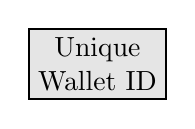
\begin{tikzpicture}
        \node [fill=gray!20,draw=black,thick,align=center] { Unique \\ Wallet ID};
      \end{tikzpicture}
    }}
    \newinst[2]{exchange}{\shortstack{Taler (exchange) \\
       \\ 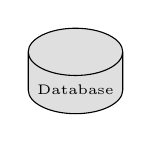
\begin{tikzpicture}[shape aspect=.5]
        \tikzset{every node/.style={cylinder,shape border rotate=90, draw,fill=gray!25}}
        \node at (1.5,0) {\shortstack{{{\tiny Database}}}};
       \end{tikzpicture}
    }}
    \newinst[2]{bank}{\shortstack{Customer bank \\
      \\ 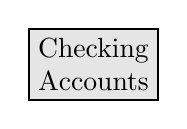
\begin{tikzpicture}
        \node [fill=gray!20,draw=black,thick,align=center] {Checking \\ Accounts};
      \end{tikzpicture}
    }}
    \postlevel
    \mess[0]{wallet}{Withdraw {(Amount)}}{exchange}
   \mess[0]{exchange}{{Configuration (ToS, Fees)}}{wallet}
    \begin{sdblock}{once}{}
      \begin{callself}{wallet}{Accept ToS}{}
      \end{callself}
    \end{sdblock}
    \begin{callself}{wallet}{Review withdraw fees}{}
    \end{callself}
    \mess[0]{wallet}{{Initiate transfer (Amount, Credit account, Wallet ID)}}{bank}
    \mess[0]{bank}{{Credit (Wallet ID)}}{exchange}

    \begin{sdblock}{Acceptable transfer?}{}
    \mess[0]{exchange}{{Bounce funds}}{bank}
    \end{sdblock}
    \postlevel
    \mess[0]{exchange}{Confirm wire transfer}{wallet}
    \mess[0]{wallet}{Request digital cash}{exchange}
    \mess[0]{exchange}{Distribute digital cash}{wallet}
    \postlevel
    \begin{sdblock}{Withdraw period expired?}{}
    \mess[0]{exchange}{{Return remaining funds}}{bank}
    \end{sdblock}
\end{sequencediagram}
  \caption{Withdraw interactions between customer, Taler exchange (payment
    service provider) and bank.  The amount of digital cash distributed is
    subject to limits per origin account (see Figure~\ref{fig:kyc:withdraw}).}
  \label{fig:int:withdraw}
\end{figure}

\section{Deposit} \label{sec:deposit}

\begin{figure}[h!]
  \begin{sequencediagram}
    \newinst{wallet}{\shortstack{Customer wallet \\
      \\ 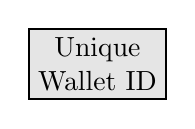
\begin{tikzpicture}
        \node [fill=gray!20,draw=black,thick,align=center] { Unique \\ Wallet ID};
      \end{tikzpicture}
    }}
    \newinst[2]{exchange}{\shortstack{Taler (exchange) \\
       \\ 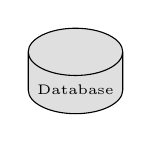
\begin{tikzpicture}[shape aspect=.5]
        \tikzset{every node/.style={cylinder,shape border rotate=90, draw,fill=gray!25}}
        \node at (1.5,0) {\shortstack{{{\tiny Database}}}};
       \end{tikzpicture}
    }}
    \newinst[2]{bank}{\shortstack{Retail bank \\
      \\ 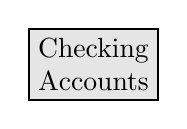
\begin{tikzpicture}
        \node [fill=gray!20,draw=black,thick,align=center] {Checking \\ Accounts};
      \end{tikzpicture}
    }}
    \postlevel
    \begin{callself}{wallet}{Review deposit fees}{}
    \end{callself}
    \mess[0]{wallet}{Deposit {(Coins)}}{exchange}
    \begin{sdblock}{Acceptable account?}{}
    \mess[0]{exchange}{{Refuse deposit}}{wallet}
    \end{sdblock}
    \begin{sdblock}{KYC/AML required?}{}
    \begin{callself}{exchange}{Figures~\ref{fig:proc:kyc}, \ref{fig:proc:aml}}{}
    \end{callself}
    \end{sdblock}
%    \prelevel
%    \prelevel
%    \begin{sdblock}{User abort?}{}
%    \mess[0]{wallet}{{Request abort}}{exchange}
%    \mess[0]{exchange}{{Abort confirmation}}{wallet}
%    \end{sdblock}
    \mess[0]{exchange}{{Initiate transfer}}{bank}

\end{sequencediagram}
  \caption{A customer deposits the coins issued by a Taler exchange (payment
    service provider) into a bank account.  Even if the
    bank account is owned by the same customer, the
    KYC checks from Section~\ref{sec:kyc:deposit} apply.}
  \label{fig:int:deposit}
\end{figure}

We do {\bf not} permit the customer to regain control over their funds {\em
  unless} they pass the KYC/AML checks. The technical reason is simply that
the KYC/AML checks happen {\em after} the aggregation logic and at this point
refunds are no longer permitted.  From a compliance perspective, this also
prevents malicious customers from risk-free probing of the system.

\section{Pay} \label{sec:pay}

\begin{figure}[h!]
  \begin{sequencediagram}
    \newinst{wallet}{\shortstack{Customer wallet \\
      \\ 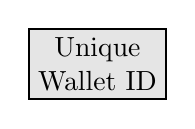
\begin{tikzpicture}
        \node [fill=gray!20,draw=black,thick,align=center] { Unique \\ Wallet ID};
      \end{tikzpicture}
    }}
    \newinst[1]{merchant}{\shortstack{Merchant \\
       \\ 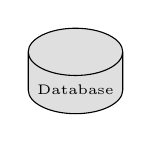
\begin{tikzpicture}[shape aspect=.5]
        \tikzset{every node/.style={cylinder,shape border rotate=90, draw,fill=gray!25}}
        \node at (1.5,0) {\shortstack{{{\tiny Database}}}};
       \end{tikzpicture}
    }}
    \newinst[1]{exchange}{\shortstack{Taler (exchange) \\
       \\ 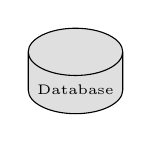
\begin{tikzpicture}[shape aspect=.5]
        \tikzset{every node/.style={cylinder,shape border rotate=90, draw,fill=gray!25}}
        \node at (1.5,0) {\shortstack{{{\tiny Database}}}};
       \end{tikzpicture}
    }}
    \newinst[1]{bank}{\shortstack{Merchant bank \\
      \\ 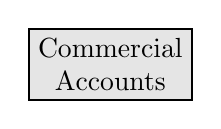
\begin{tikzpicture}
        \node [fill=gray!20,draw=black,thick,align=center] {Commercial \\ Accounts};
      \end{tikzpicture}
    }}
    \postlevel
    \mess[0]{wallet}{Browse catalog}{merchant}
    \mess[0]{merchant}{Commercial offer}{wallet}
    \begin{callself}{wallet}{Review offer}{}
    \end{callself}
    \mess[0]{wallet}{Pay {(Coins)}}{merchant}
    \prelevel
    \mess[0]{merchant}{Deposit {(Coins)}}{exchange}
    \begin{sdblock}{KYC/AML required?}{}
    \begin{callself}{exchange}{Figures~\ref{fig:proc:kyc}, \ref{fig:proc:aml}}{}
    \end{callself}
    \end{sdblock}
    \begin{sdblock}{Acceptable account?}{}
    \mess[0]{exchange}{{Refuse deposit}}{merchant}
    \prelevel
    \mess[0]{merchant}{{Fail purchase}}{wallet}
    \end{sdblock}
    \mess[0]{exchange}{{Confirm deposit}}{merchant}
    \prelevel
    \mess[0]{merchant}{Fulfill order}{wallet}
    \begin{callself}{exchange}{Aggregate transactions}{}
    \end{callself}
    \begin{sdblock}{KYC/AML required?}{}
    \begin{callself}{exchange}{Figures~\ref{fig:proc:kyc}, \ref{fig:proc:aml}}{}
    \end{callself}
    \end{sdblock}
    \mess[0]{exchange}{{Initiate transfer}}{bank}
  \end{sequencediagram}
  \caption{Payments from a customer to merchant result in
    depositing coins at the Taler exchange (payment service provider)
    which then credits the merchant's bank account.
    The KYC/AML checks are described in Section~\ref{sec:kyc:deposit}}
  \label{fig:int:pay}
\end{figure}

{\bf Internal note:} The exchange refusing a deposit immediately based on
unaccaptable merchant accounts can depend both on the target account
(e.g. wire method not supported) or on the legitimization state of the
merchant's target account (including lack of KYC authorization wire
transfer, failure to accept terms of service, failure to provide KYC
data, or some kind of AML/KYC rule being violated).  However, in general
the merchant backend will know if it has performed some mandatory sign-up
process and can thus avoid the entire situation by only offering exchanges
where the merchant is in good standing in its contracts.  The central
bug for supporting this in the merchant is \#9052.

\section{Refund}

\begin{figure}[h!]
  \begin{sequencediagram}
    \newinst{wallet}{\shortstack{Customer wallet \\
      \\ 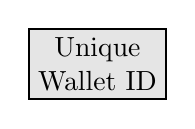
\begin{tikzpicture}
        \node [fill=gray!20,draw=black,thick,align=center] { Unique \\ Wallet ID};
      \end{tikzpicture}
    }}
    \newinst[2]{merchant}{\shortstack{Merchant \\
       \\ 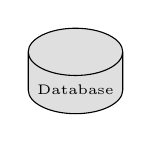
\begin{tikzpicture}[shape aspect=.5]
        \tikzset{every node/.style={cylinder,shape border rotate=90, draw,fill=gray!25}}
        \node at (1.5,0) {\shortstack{{{\tiny Database}}}};
       \end{tikzpicture}
    }}
    \newinst[2]{exchange}{\shortstack{Taler (exchange) \\
       \\ 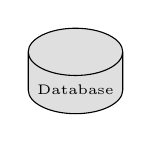
\begin{tikzpicture}[shape aspect=.5]
        \tikzset{every node/.style={cylinder,shape border rotate=90, draw,fill=gray!25}}
        \node at (1.5,0) {\shortstack{{{\tiny Database}}}};
       \end{tikzpicture}
    }}
    \postlevel
    \begin{callself}{merchant}{Initiate refund}{}
    \end{callself}
    \mess[0]{merchant}{{Refund offer (QR code)}}{wallet}
    \mess[0]{wallet}{Download refund}{merchant}
    \mess[0]{merchant}{Approve refund}{exchange}
    \mess[0]{exchange}{Confirm refund}{merchant}
    \mess[0]{merchant}{Return refund confirmation}{wallet}
  \end{sequencediagram}
  \caption{Refund processing when a merchant is unable to fulfill
    a contract.  Refunds must happen {\em before} the
    exchange has aggregated the original transaction for
    a bank transfer to the merchant. Furthermore, refunds
    can only go to the customer who made the original payment
    and the refund cannot exceed the amount of the original
    payment.}
  \label{fig:int:refund}
\end{figure}

\section{Push payment}

\begin{figure}[h!]
  \begin{sequencediagram}
    \newinst{payer}{\shortstack{Payer \\
      \\ 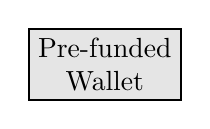
\begin{tikzpicture}
        \node [fill=gray!20,draw=black,thick,align=center] {Pre-funded \\ Wallet};
      \end{tikzpicture}
    }}
    \newinst[2]{exchange}{\shortstack{Taler (exchange) \\
       \\ 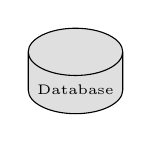
\begin{tikzpicture}[shape aspect=.5]
        \tikzset{every node/.style={cylinder,shape border rotate=90, draw,fill=gray!25}}
        \node at (1.5,0) {\shortstack{{{\tiny Database}}}};
       \end{tikzpicture}
    }}
    \newinst[2]{payee}{\shortstack{Payee \\
      \\ 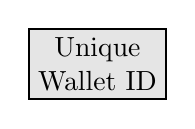
\begin{tikzpicture}
        \node [fill=gray!20,draw=black,thick,align=center] { Unique \\ Wallet ID};
      \end{tikzpicture}
    }}
    \postlevel
    \begin{callself}{payer}{Review push payment fees}{}
    \end{callself}
    \mess[0]{payer}{{Push funds (Coins)}}{exchange}
    \mess[0]{payer}{{Offer payment (e.g. via QR code)}}{payee}
    \begin{callself}{payee}{Review payment offer}{}
    \end{callself}
    \mess[0]{payee}{{Request funds (Wallet ID)}}{exchange}
    \begin{sdblock}{Domestic wallet?}{}
    \begin{callself}{exchange}{Figure~\ref{fig:proc:domestic}}{}
    \end{callself}
    \end{sdblock}
    \begin{sdblock}{KYC/AML required?}{}
    \begin{callself}{exchange}{Figures~\ref{fig:proc:kyc}, \ref{fig:proc:aml}}{}
    \end{callself}
    \end{sdblock}
    \mess[0]{exchange}{{Distribute digital cash}}{payee}
%    \postlevel
    \begin{sdblock}{Payment offer expired?}{}
    \mess[0]{exchange}{{Return funds}}{payer}
    \end{sdblock}

\end{sequencediagram}
  \caption{Interactions between wallets and Taler exchange
    in a push payment.}
  \label{fig:int:push}
\end{figure}

\section{Pull payment (aka invoicing)}

\begin{figure}[h!]
  \begin{sequencediagram}
    \newinst{payer}{\shortstack{Payer \\
      \\ 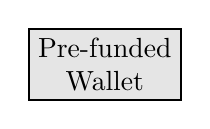
\begin{tikzpicture}
        \node [fill=gray!20,draw=black,thick,align=center] {Pre-funded \\ Wallet};
      \end{tikzpicture}
    }}
    \newinst[2]{exchange}{\shortstack{Taler (exchange) \\
       \\ 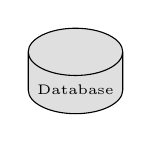
\begin{tikzpicture}[shape aspect=.5]
        \tikzset{every node/.style={cylinder,shape border rotate=90, draw,fill=gray!25}}
        \node at (1.5,0) {\shortstack{{{\tiny Database}}}};
       \end{tikzpicture}
    }}
    \newinst[2]{payee}{\shortstack{Payee \\
      \\ 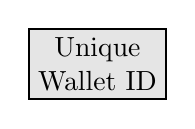
\begin{tikzpicture}
        \node [fill=gray!20,draw=black,thick,align=center] { Unique \\ Wallet ID};
      \end{tikzpicture}
    }}
    \postlevel
    \begin{callself}{payee}{Review pull payment fees}{}
    \end{callself}
    \mess[0]{payee}{{Create invoice (Wallet ID)}}{exchange}

    \mess[0]{exchange}{{Invoice ready}}{payee}
    \mess[0]{payee}{{Send invoice (e.g. via QR code)}}{payer}

    \begin{callself}{payer}{Review invoice}{}
    \end{callself}
    \mess[0]{payer}{{Make payment (Coins)}}{exchange}

    \begin{sdblock}{Domestic wallet?}{}
    \begin{callself}{exchange}{Figure~\ref{fig:proc:domestic}}{}
    \end{callself}
    \end{sdblock}
    \begin{sdblock}{KYC/AML required?}{}
    \begin{callself}{exchange}{Figures~\ref{fig:proc:kyc}, \ref{fig:proc:aml}}{}
    \end{callself}
    \end{sdblock}

    \mess[0]{exchange}{{Distribute digital cash}}{payee}

\end{sequencediagram}
  \caption{Interactions between wallets and Taler exchange
    in a pull payment.}
  \label{fig:int:pull}
\end{figure}

We do {\bf not} permit the payer to regain control over their funds, once the
payment was made they are locked {\em until} the payee passes the KYC/AML
checks.  We only do the AML/KYC process once the funds are locked at the
exchange. This ensures we know the actual transacted amounts (which may be
lower than the total amounts requested) and prevents risk-free probing
attacks.

\section{Shutdown}

\begin{figure}[h!]
  \begin{sequencediagram}
    \newinst{wallet}{\shortstack{Customer wallet \\
      \\ 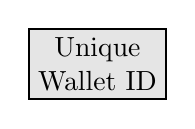
\begin{tikzpicture}
        \node [fill=gray!20,draw=black,thick,align=center] { Unique \\ Wallet ID};
      \end{tikzpicture}
    }}
    \newinst[2]{exchange}{\shortstack{Taler (exchange) \\
       \\ 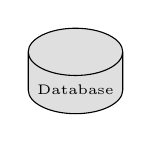
\begin{tikzpicture}[shape aspect=.5]
        \tikzset{every node/.style={cylinder,shape border rotate=90, draw,fill=gray!25}}
        \node at (1.5,0) {\shortstack{{{\tiny Database}}}};
       \end{tikzpicture}
    }}
    \newinst[2]{bank}{\shortstack{Customer bank \\
      \\ 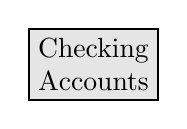
\begin{tikzpicture}
        \node [fill=gray!20,draw=black,thick,align=center] {Checking \\ Accounts};
      \end{tikzpicture}
    }}
    \postlevel

    \begin{callself}{exchange}{Operator initiates shutdown}{}
    \end{callself}
     \mess[0]{exchange}{{Shutdown alert}}{wallet}
     \begin{sdblock}{Bank account known?}{}
       \begin{callself}{wallet}{Designate bank account}{}
       \end{callself}
     \end{sdblock}
    \mess[0]{wallet}{{Deposit (Coins)}}{exchange}
    \begin{sdblock}{Acceptable account?}{}
    \mess[0]{exchange}{{Refuse deposit}}{wallet}
    \end{sdblock}
    \begin{sdblock}{KYC/AML required?}{}
    \begin{callself}{exchange}{Figures~\ref{fig:proc:kyc}, \ref{fig:proc:aml}}{}
    \end{callself}
    \end{sdblock}
    \mess[0]{exchange}{{Initiate transfer}}{bank}
\end{sequencediagram}
  \caption{Shutdown interactions between customer, Taler exchange (payment
    service provider) and bank.}
  \label{fig:int:shutdown}
\end{figure}

KYC/AML requirements are relaxed in cases where the customer is able to
cryptographically demonstrate that they previously withdrew these coins from
the designated checking account.  Thus, KYC/AML checks here primarily still
apply if the customer received the funds via P2P transfers from other wallets.



\chapter{Regulatory Triggers} \label{chap:triggers}

In this chapter we show decision diagrams for regulatory processes of the
various core operations of the GNU Taler payment system.  In each case, the
{\bf start} state refers to one of the interactions described in the previous
chapter.  The payment system will then use the process to arrive at an {\bf
  allow} decision which permits the transaction to go through, or at a {\bf
  deny} decision which ensures that the funds are not moved.

The specific {\em decisions} (in green) depend on the risk profile and the
regulatory environment. The tables in each section list the specific values
that are to be configured.

There are five types if interactions that can trigger regulatory processes:

\begin{description}
  \item[withdraw] a customer withdraws digital cash from their {\bf bank account}
  \item[deposit] a merchant's {\bf bank account} is designated to receive a payment in digital cash
  \item[push] a {\bf wallet} accepts a payment from another wallet
  \item[pull] a {\bf wallet} requests a payment from another wallet
%  \item[balance] a withdraw or P2P payment causes the balance of a {\bf wallet} to exceed a given threshold
\end{description}

We note in bold the {\bf anchor} for the regulator process. The anchor is used
to link the interaction to an identity.  Once an identity has been established
for a particular anchor, that link is considered established for all types of
activities involving that anchor.  A wallet is uniquely identified in the
system by its unique cryptographic key.  A bank account is uniquely identified
in the system by its (RFC 8905) bank routing data (usually including BIC, IBAN
and account owner name).

The KYC and AML processes themselves are described in
Chapter~\ref{chap:regproc}.

\section{KYC: Withdraw} \label{sec:kyc:withdraw}

\begin{figure}[h!]
  \begin{center}
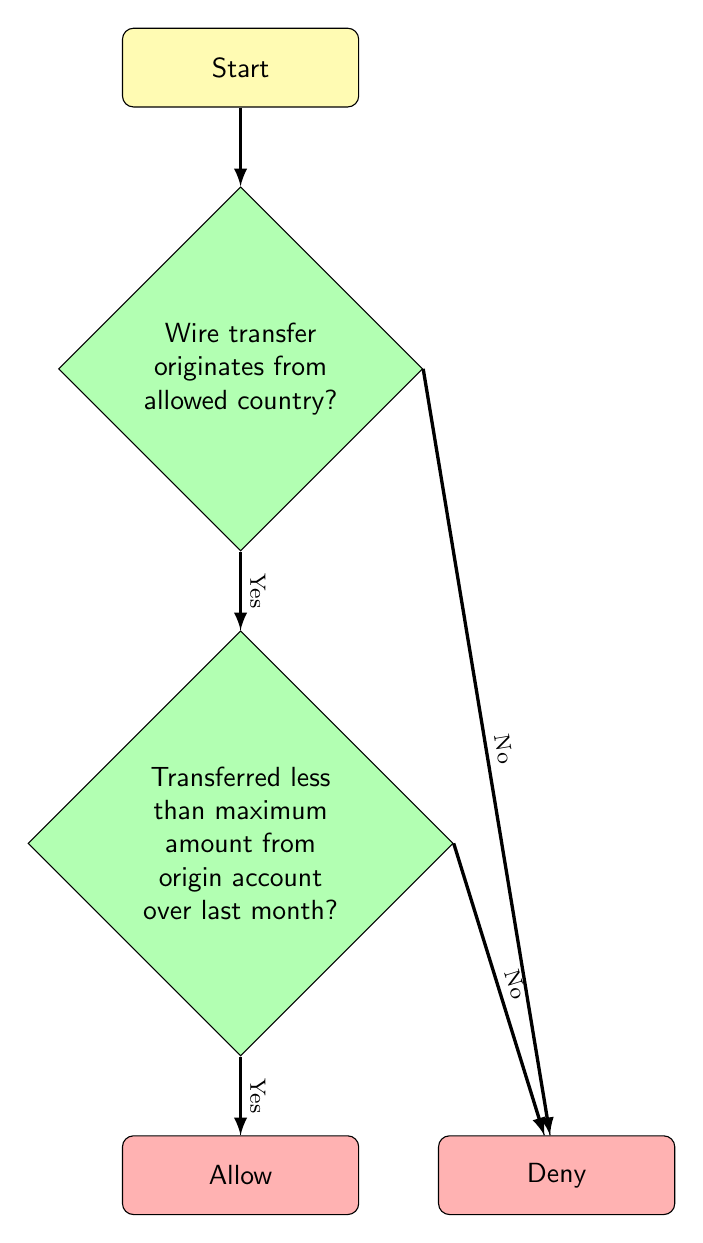
\begin{tikzpicture}[node distance=1cm,font=\sffamily,
    start/.style={rectangle, rounded corners, minimum width=3cm, minimum height=1cm,text centered, draw=black, fill=yellow!30},
    end/.style={rectangle, rounded corners, minimum width=3cm, minimum height=1cm,text centered, draw=black, fill=red!30},
    process/.style={rectangle, minimum width=3cm, minimum height=1cm, text centered, draw=black, fill=orange!30},
    failed/.style={rectangle, rounded corners, minimum width=3cm, minimum height=1cm, text centered, draw=black, fill=red!30},
    io/.style={trapezium, trapezium left angle=70, trapezium right angle=110, minimum width=3cm, minimum height=1cm, text centered, draw=black, fill=blue!30},
    decision/.style={diamond, minimum width=3cm, minimum height=1cm, text centered, draw=black, fill=green!30},
    arr/.style={very thick,-latex},
    every edge quotes/.style = {auto, font=\footnotesize, sloped}
    ]
 \node (start) [start] {Start};
 \node (country) [decision,below=of start,text width=3cm] {Wire transfer originates from allowed country?};
 \node (amount) [decision, below=of country,text width=3cm] {Transferred less than maximum amount from origin account over last month?};
 \node (allow) [end, below=of amount] {Allow};
 \node (deny) [failed, right=of allow] {Deny};
 \draw[arr] (start) -> (country) {};
 \draw[arr] (country) -> (amount);
 \draw (country) edge["Yes"] (amount);
 \draw[arr] (country.east) -> (deny);
 \draw (country.east) edge["No"] (deny);
 \draw[arr] (amount) -> (allow);
 \draw (amount) edge["Yes"] (allow);
 \draw[arr] (amount.east) -> (deny);
 \draw (amount.east) edge["No"] (deny);
\end{tikzpicture}
  \end{center}
  \caption{Regulatory process when withdrawing digital cash from a
    bank account.
    If the transfer is denied or the user fails to withdraw the
    funds for any other reason, the money is automatically returned
    after the bounce period (see Table~\ref{table:kyc:withdraw:settings}) to
    the originating bank account.}
  \label{fig:kyc:withdraw}
\end{figure}

\begin{table}[h!]
  \caption{Settings for the withdraw trigger. Note that the operation
  must satisfy all of the given rules.} \label{table:kyc:withdraw:settings}
  \begin{tabular}{l|l|r}
    {\bf Setting}            & {\bf Type}         &  {\bf Value}     \\ \hline \hline
    Allowed bank accounts    & RFC 8905 RegEx     &  {\em CH*}       \\ \hline
    SMS-Identification       & Amount/month       &  {\em 200 CHF}   \\
    Withdraw limit           & Amount/month       &  {\em 5000 CHF}  \\
    Withdraw limit           & Amount/year        &  {\em 15000 CHF} \\
    Bounce period            & Delay              &  1 month         \\
  \end{tabular}
\end{table}

%The limit of 200 \CURRENCY{} results from article 48-2.  Strictly limiting
%withdrawals to less than 5'000 \CURRENCY{} per month and less than 15'000
%\CURRENCY{} per year assures compliance with article 48-1c.

SMS-Identification is done by in-house software.  Withdraw limits are
hard and cannot be raised even if the customer is known.

\section{KYC: Deposit} \label{sec:kyc:deposit}

\begin{figure}[h!]
  \begin{center}
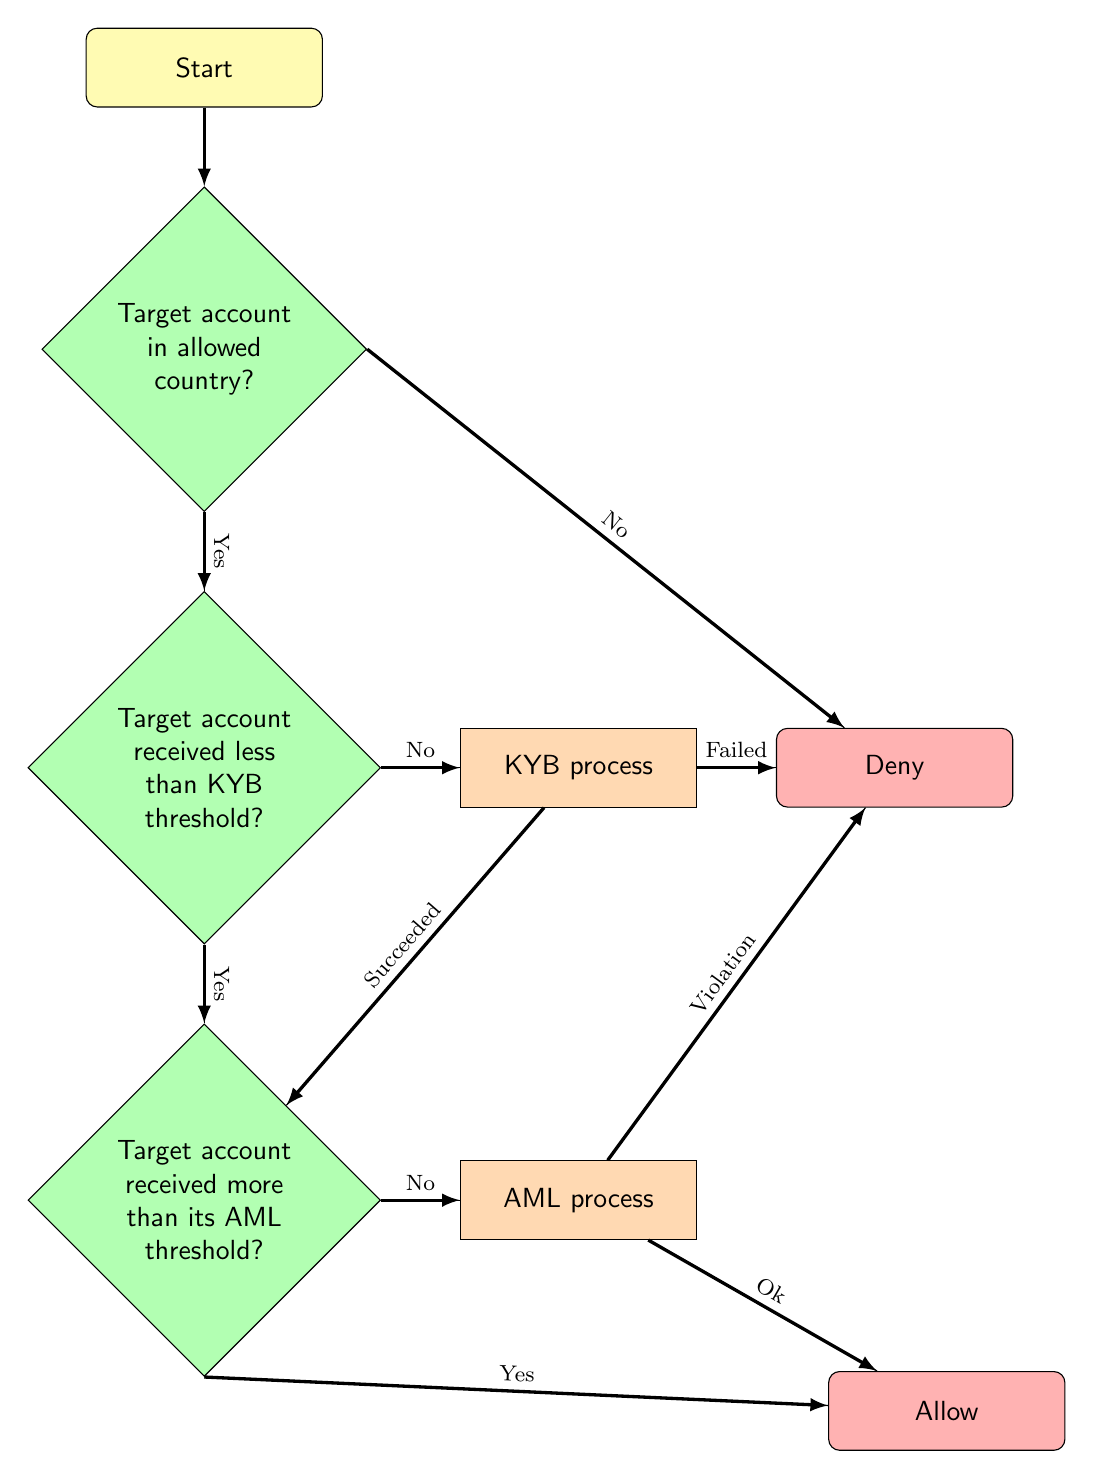
\begin{tikzpicture}[node distance=1cm,font=\sffamily,
    start/.style={rectangle, rounded corners, minimum width=3cm, minimum height=1cm,text centered, draw=black, fill=yellow!30},
    end/.style={rectangle, rounded corners, minimum width=3cm, minimum height=1cm,text centered, draw=black, fill=red!30},
    process/.style={rectangle, minimum width=3cm, minimum height=1cm, text centered, draw=black, fill=orange!30},
    failed/.style={rectangle, rounded corners, minimum width=3cm, minimum height=1cm, text centered, draw=black, fill=red!30},
    io/.style={trapezium, trapezium left angle=70, trapezium right angle=110, minimum width=3cm, minimum height=1cm, text centered, draw=black, fill=blue!30},
    decision/.style={diamond, minimum width=3cm, minimum height=1cm, text centered, draw=black, fill=green!30},
    arr/.style={very thick,-latex},
    every edge quotes/.style = {auto, font=\footnotesize, sloped}
    ]
 \node (start) [start] {Start};
 \node (country) [decision,below=of start,text width=2.5cm] {Target account in allowed country?};
 \node (amount) [decision, below=of country,text width=2.5cm] {Target account received less than KYB threshold?};
 \node (kyc) [process, right=of amount] {KYB process};
 \node (high) [decision, below=of amount,text width=2.5cm] {Target account received more than its AML threshold?};
 \node (aml) [process, right=of high] {AML process};
 \node (dummy) [below right=of aml] {};
 \node (allow) [end, below right=of dummy] {Allow};
 \node (deny) [failed, right=of kyc] {Deny};
 \draw[arr] (start) -> (country) {};

 \draw[arr] (country) -> (amount);
 \draw (country) edge["Yes"] (amount);

 \draw[arr] (country.east) -> (deny);
 \draw (country.east) edge["No"] (deny);

 \draw[arr] (amount) -> (high);
 \draw (amount) edge["Yes"] (high);

 \draw[arr] (amount.east) -> (kyc);
 \draw (amount.east) edge["No"] (kyc);

 \draw[arr] (kyc) -> (deny);
 \draw (kyc) edge["Failed"] (deny);

 \draw[arr] (kyc) -> (high);
 \draw (kyc) edge["Succeeded"] (high);

 \draw[arr] (high.south) -> (allow);
 \draw (high.south) edge["Yes"] (allow);

 \draw[arr] (high.east) -> (aml);
 \draw (high.east) edge["No"] (aml);

 \draw[arr] (aml) -> (deny);
 \draw (aml) edge["Violation"] (deny);

 \draw[arr] (aml) -> (allow);
 \draw (aml) edge["Ok"] (allow);
\end{tikzpicture}
  \end{center}
  \caption{Regulatory process when depositing digital cash into a bank
    account.  When the transfer is denied, the money is held in escrow
    until authorities authorize the transfer.}
\end{figure}


\begin{table}[h!]
  \caption{Settings for the deposit trigger. Note that the operation
  must satisfy all of the given rules.}
  \begin{tabular}{l|l|r}
    {\bf Setting}                 & {\bf Type}         & {\bf Value}     \\ \hline \hline
    Allowed bank accounts         & RFC 8905 RegEx     & {\em CH*}       \\ \hline
    KYB deposit threshold         & Amount/month       & {\em  5000 CHF} \\
    KYB deposit threshold         & Amount/year        & {\em 25000 CHF} \\
    Default AML deposit threshold & Amount/month       & {\em  5000 CHF} \\
  \end{tabular}
\end{table}

The KYB deposit threshold of 5'000 \CURRENCY{} per month and than 25'000
\CURRENCY{} per year ensure compliance with article 48-1b.

Additionally, our terms of service will prohibit businesses to receive
amounts exceeding 1'000 \CURRENCY{} per transaction (well below the
15'000 \CURRENCY{} threshold defined in article 24-1c).

SMS-Identification is done by in-house software. KYB data is initially
obtained and vetted by one of several external KYB providers before
being passed for manual validation by our own staff who can then
determine appropriate AML thresholds and set review criteria.

\section{KYC/AML: Push Payment} \label{sec:kyc:push}

\begin{figure}[h!]
  \begin{center}
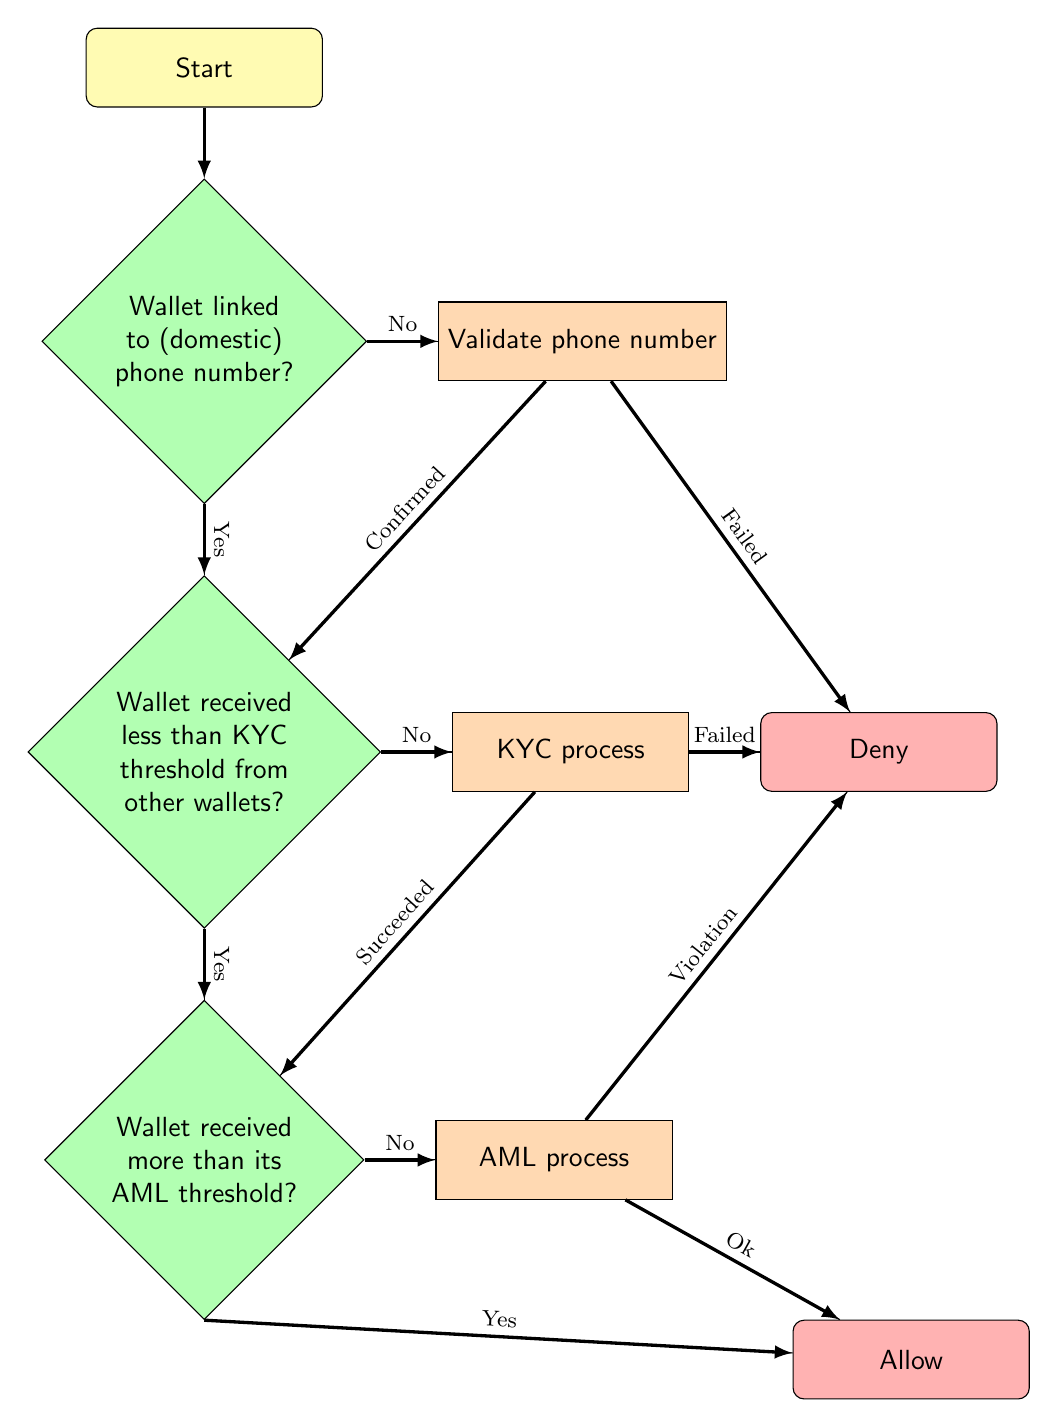
\begin{tikzpicture}[node distance=0.9cm,font=\sffamily,
    start/.style={rectangle, rounded corners, minimum width=3cm, minimum height=1cm,text centered, draw=black, fill=yellow!30},
    end/.style={rectangle, rounded corners, minimum width=3cm, minimum height=1cm,text centered, draw=black, fill=red!30},
    process/.style={rectangle, minimum width=3cm, minimum height=1cm, text centered, draw=black, fill=orange!30},
    failed/.style={rectangle, rounded corners, minimum width=3cm, minimum height=1cm, text centered, draw=black, fill=red!30},
    io/.style={trapezium, trapezium left angle=70, trapezium right angle=110, minimum width=3cm, minimum height=1cm, text centered, draw=black, fill=blue!30},
    decision/.style={diamond, minimum width=3cm, minimum height=1cm, text centered, draw=black, fill=green!30},
    arr/.style={very thick,-latex},
    every edge quotes/.style = {auto, font=\footnotesize, sloped}
    ]
 \node (start) [start] {Start};
 \node (wallet) [decision,below=of start,text width=2.5cm] {Wallet linked to (domestic) phone number?};
 \node (domestic) [process, right=of wallet] {Validate phone number};
 \node (amount) [decision, below=of wallet,text width=2.5cm] {Wallet received less than KYC threshold from other wallets?};
 \node (kyc) [process, right=of amount] {KYC process};
 \node (high) [decision, below=of amount,text width=2.5cm] {Wallet received more than its AML threshold?};
 \node (aml) [process, right=of high] {AML process};
 \node (dummy) [below right=of aml] {};
 \node (allow) [end, below right=of dummy] {Allow};
 \node (deny) [failed, right=of kyc] {Deny};
 \draw[arr] (start) -> (wallet) {};

 \draw[arr] (wallet) -> (amount);
 \draw (wallet) edge["Yes"] (amount);

 \draw[arr] (wallet.east) -> (domestic);
 \draw (wallet.east) edge["No"] (domestic);

 \draw[arr] (domestic) -> (amount);
 \draw (domestic) edge["Confirmed"] (amount);

 \draw[arr] (domestic) -> (deny);
 \draw (domestic) edge["Failed"] (deny);

 \draw[arr] (amount) -> (high);
 \draw (amount) edge["Yes"] (high);

 \draw[arr] (amount.east) -> (kyc);
 \draw (amount.east) edge["No"] (kyc);

 \draw[arr] (kyc) -> (deny);
 \draw (kyc) edge["Failed"] (deny);

 \draw[arr] (kyc) -> (high);
 \draw (kyc) edge["Succeeded"] (high);

 \draw[arr] (high.south) -> (allow);
 \draw (high.south) edge["Yes"] (allow);

 \draw[arr] (high.east) -> (aml);
 \draw (high.east) edge["No"] (aml);

 \draw[arr] (aml) -> (deny);
 \draw (aml) edge["Violation"] (deny);

 \draw[arr] (aml) -> (allow);
 \draw (aml) edge["Ok"] (allow);
\end{tikzpicture}
  \end{center}
  \caption{Regulatory process when receiving payments from another wallet.
    The threshold depends on the risk profile from the KYC process.
    When the transfer is denied the money is (eventually) returned to
    the originating wallet.}
\end{figure}


\begin{table}[h!]
  \caption{Settings for the push payment trigger. Note that the operation
  must satisfy all of the given rules.}
  \begin{tabular}{l|l|r}
    {\bf Setting}             & {\bf Type}     & {\bf Value} \\ \hline \hline
    Permitted phone numbers   & Dialing prefix & {\em +41} \\
    P2P KYC threshold         & Amount/month   & {\em  1000 CHF} \\
    P2P KYC threshold         & Amount/year    & {\em  5000 CHF} \\
    Default P2P AML threshold & Amount/month   & {\em  2500 CHF} \\
  \end{tabular}
\end{table}

The P2P KYC thresholds of 1'000 \CURRENCY{} per month and than 5'000
\CURRENCY{} per year ensure compliance with article 49-2c.

\section{KYC/AML: Pull Payment}

\begin{figure}[h!]
  \begin{center}
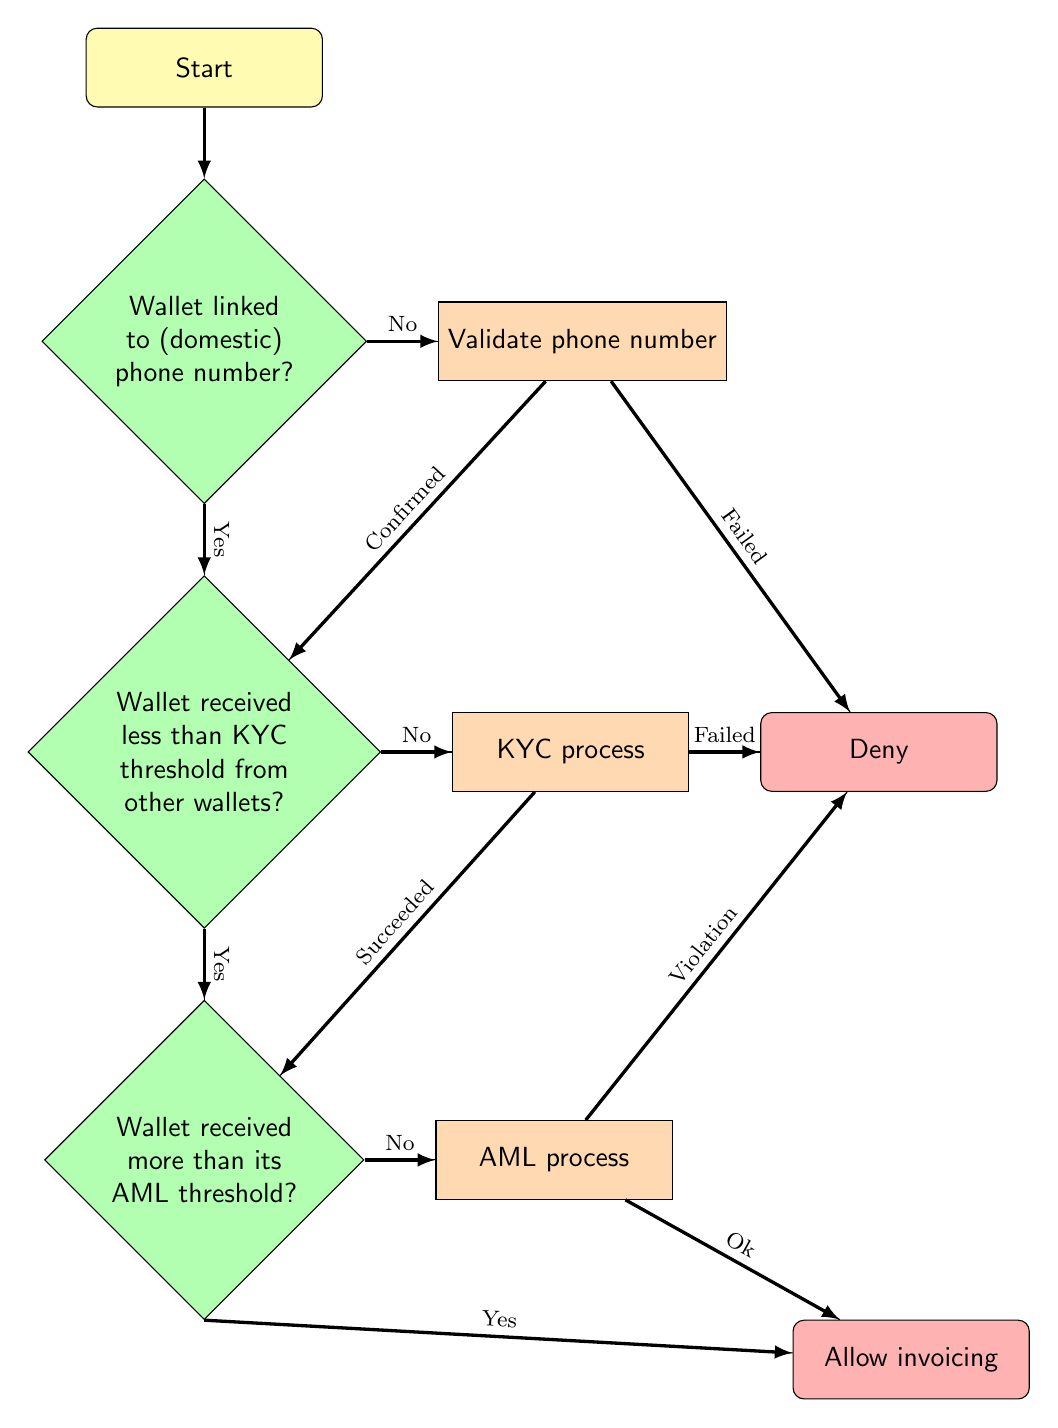
\begin{tikzpicture}[node distance=0.9cm,font=\sffamily,
    start/.style={rectangle, rounded corners, minimum width=3cm, minimum height=1cm,text centered, draw=black, fill=yellow!30},
    end/.style={rectangle, rounded corners, minimum width=3cm, minimum height=1cm,text centered, draw=black, fill=red!30},
    process/.style={rectangle, minimum width=3cm, minimum height=1cm, text centered, draw=black, fill=orange!30},
    failed/.style={rectangle, rounded corners, minimum width=3cm, minimum height=1cm, text centered, draw=black, fill=red!30},
    io/.style={trapezium, trapezium left angle=70, trapezium right angle=110, minimum width=3cm, minimum height=1cm, text centered, draw=black, fill=blue!30},
    decision/.style={diamond, minimum width=3cm, minimum height=1cm, text centered, draw=black, fill=green!30},
    arr/.style={very thick,-latex},
    every edge quotes/.style = {auto, font=\footnotesize, sloped}
    ]
 \node (start) [start] {Start};
 \node (wallet) [decision,below=of start,text width=2.5cm] {Wallet linked to (domestic) phone number?};
 \node (domestic) [process, right=of wallet] {Validate phone number};
 \node (amount) [decision, below=of wallet,text width=2.5cm] {Wallet received less than KYC threshold from other wallets?};
 \node (kyc) [process, right=of amount] {KYC process};
 \node (high) [decision, below=of amount,text width=2.5cm] {Wallet received more than its AML threshold?};
 \node (aml) [process, right=of high] {AML process};
 \node (dummy) [below right=of aml] {};
 \node (allow) [end, below right=of dummy] {Allow invoicing};
 \node (deny) [failed, right=of kyc] {Deny};
 \draw[arr] (start) -> (wallet) {};

 \draw[arr] (wallet) -> (amount);
 \draw (wallet) edge["Yes"] (amount);

 \draw[arr] (wallet.east) -> (domestic);
 \draw (wallet.east) edge["No"] (domestic);

 \draw[arr] (domestic) -> (amount);
 \draw (domestic) edge["Confirmed"] (amount);

 \draw[arr] (domestic) -> (deny);
 \draw (domestic) edge["Failed"] (deny);

 \draw[arr] (amount) -> (high);
 \draw (amount) edge["Yes"] (high);

 \draw[arr] (amount.east) -> (kyc);
 \draw (amount.east) edge["No"] (kyc);

 \draw[arr] (kyc) -> (deny);
 \draw (kyc) edge["Failed"] (deny);

 \draw[arr] (kyc) -> (high);
 \draw (kyc) edge["Succeeded"] (high);

 \draw[arr] (high.south) -> (allow);
 \draw (high.south) edge["Yes"] (allow);

 \draw[arr] (high.east) -> (aml);
 \draw (high.east) edge["No"] (aml);

 \draw[arr] (aml) -> (deny);
 \draw (aml) edge["Violation"] (deny);

 \draw[arr] (aml) -> (allow);
 \draw (aml) edge["Ok"] (allow);
\end{tikzpicture}
  \end{center}
  \caption{Regulatory process when receiving payments from another wallet.
    The threshold depends on the risk profile from the KYC process.
    When invoicing is denied the wallet cannot generate the invoice.}
\end{figure}


\begin{table}[h!]
  \caption{Settings for the pull payment trigger. Note that the operation
  must satisfy all of the given rules.}
  \begin{tabular}{l|l|r}
    {\bf Setting}             & {\bf Type}      & {\bf Value} \\ \hline \hline
    Permitted phone numbers   & Dialing prefix  & {\em +41} \\
    P2P KYC threshold         & Amount/month    & {\em  1000 CHF} \\
    P2P KYC threshold         & Amount/year     & {\em  5000 CHF} \\
    Default P2P AML threshold & Amount/month    & {\em  2500 CHF} \\
  \end{tabular}
\end{table}

The P2P KYC thresholds of 1'000 \CURRENCY{} per month and than 5'000
\CURRENCY{} per year ensure compliance with article 49-2c.

%\section{KYC: Balance}

Note: this process is not implemented and would require non-trivial extra work
if required.

\begin{figure}[h!]
  \begin{center}
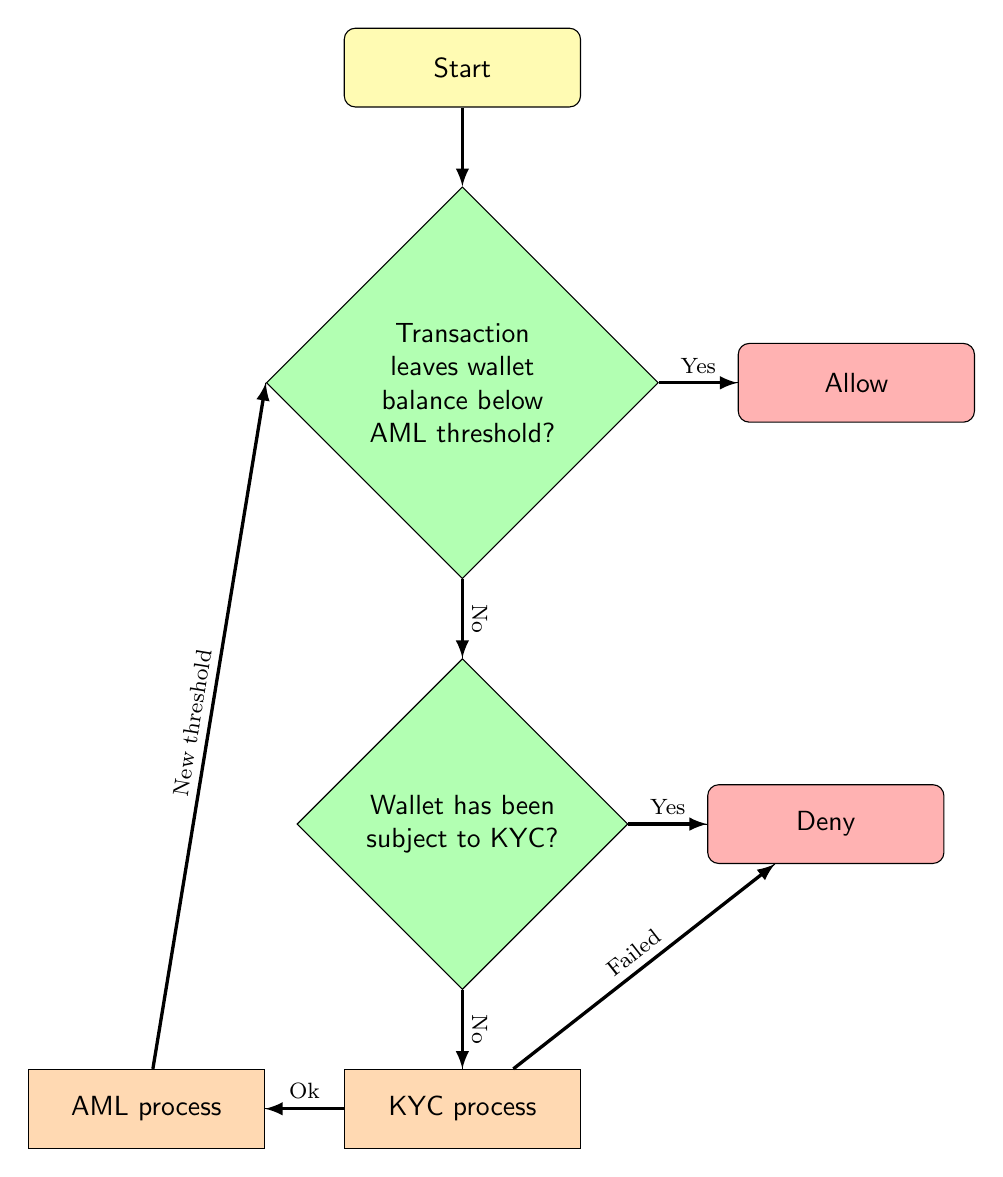
\begin{tikzpicture}[node distance=1cm,font=\sffamily,
    start/.style={rectangle, rounded corners, minimum width=3cm, minimum height=1cm,text centered, draw=black, fill=yellow!30},
    end/.style={rectangle, rounded corners, minimum width=3cm, minimum height=1cm,text centered, draw=black, fill=red!30},
    process/.style={rectangle, minimum width=3cm, minimum height=1cm, text centered, draw=black, fill=orange!30},
    failed/.style={rectangle, rounded corners, minimum width=3cm, minimum height=1cm, text centered, draw=black, fill=red!30},
    io/.style={trapezium, trapezium left angle=70, trapezium right angle=110, minimum width=3cm, minimum height=1cm, text centered, draw=black, fill=blue!30},
    decision/.style={diamond, minimum width=3cm, minimum height=1cm, text centered, draw=black, fill=green!30},
    arr/.style={very thick,-latex},
    every edge quotes/.style = {auto, font=\footnotesize, sloped}
    ]
 \node (start) [start] {Start};
 \node (balance) [decision,below=of start,text width=3cm] {Transaction leaves wallet balance below AML threshold?};
 \node (registered) [decision,below=of balance,text width=3cm] {Wallet has been subject to KYC?};
 \node (kyc) [process, below=of registered] {KYC process};
 \node (aml) [process, left=of kyc] {AML process};
 \node (allow) [end, right=of balance] {Allow};
 \node (deny) [failed, right=of registered] {Deny};
 \draw[arr] (start) -> (balance) {};
 \draw[arr] (balance) -> (registered);
 \draw (balance) edge["No"] (registered);
 \draw[arr] (balance) -> (allow);
 \draw (balance) edge["Yes"] (allow);

 \draw[arr] (registered) -> (kyc);
 \draw (registered) edge["No"] (kyc);
 \draw[arr] (registered) -> (deny);
 \draw (registered) edge["Yes"] (deny);

 \draw[arr] (kyc) -> (deny);
 \draw (kyc) edge["Failed"] (deny);
 \draw[arr] (kyc) -> (aml);
 \draw (kyc) edge["Ok"] (aml);

 \draw[arr] (aml) -> (balance.west);
 \draw (aml) edge["New threshold"] (balance.west);
\end{tikzpicture}
  \end{center}
  \caption{Regulatory process when a wallet exceeds its AML threshold.
    When the transfer is denied the transaction (withdraw, P2P transfer)
    is refused by the wallet.}
\end{figure}


\begin{table}[h!]
  \caption{Settings for the balance trigger.}
  \begin{tabular}{l|l|r}
    {\bf Setting}          & {\bf Type}         & {\bf Value} \\ \hline \hline
    KYC threshold          & Amount             & {\em 5000 CHF} \\
    Default AML threshold  & Amount             & {\em 5000 CHF} \\
  \end{tabular}
\end{table}


\chapter{Regulatory Processes} \label{chap:regproc}

This chapter describes the interactions between the customer, exchange and
organizations or staff assisting with regulatory processes designed to ensure
that customers are residents in the area of operation of the payment service
provider, are properly identified, and do not engage in money laundering.

The three main regulatory processes are:

\begin{description}
\item[domestic check] This process establishes that a user is generally
  eligible to use the payment system.  The process checks that the user has an
  eligible address, but stops short of establishing the user's identity.
\item[kyc] This process establishes a user's legal identity, possibly
  using external providers to review documents and check against blacklists.
\item[aml] The AML process reviews suspicious payment activities for
  money laundering. Here AML staff reviews all collected information.
\end{description}

\section{Domestic wallet check}

\begin{figure}[h!]
  \begin{sequencediagram}
    \newinst{wallet}{\shortstack{Customer wallet \\
      \\ 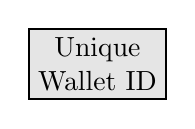
\begin{tikzpicture}
        \node [fill=gray!20,draw=black,thick,align=center] { Unique \\ Wallet ID};
      \end{tikzpicture}
    }}
    \newinst[2]{exchange}{\shortstack{Taler (exchange) \\
       \\ 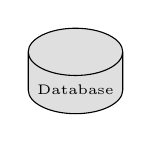
\begin{tikzpicture}[shape aspect=.5]
        \tikzset{every node/.style={cylinder,shape border rotate=90, draw,fill=gray!25}}
        \node at (1.5,0) {\shortstack{{{\tiny Database}}}};
       \end{tikzpicture}
    }}
    \newinst[2]{sms}{\shortstack{Address validator}}

    \postlevel
    \mess[0]{wallet}{{P2P payment (Wallet ID)}}{exchange}
    \begin{callself}{exchange}{New wallet?}{}
    \end{callself}
    \mess[0]{exchange}{Request address validation}{sms}
    \mess[0]{sms}{Validation process ID}{exchange}
    \mess[0]{exchange}{Request address validation}{wallet}
    \mess[0]{wallet}{Send address}{sms}
    \mess[0]{sms}{{Send confirmation code (to address)}}{wallet}
    \mess[0]{wallet}{Supply confirmation code}{sms}
    \mess[0]{sms}{{Confirmed customer address}}{exchange}
    \mess[0]{exchange}{{Confirm completion}}{wallet}
    \mess[0]{wallet}{{Retry action}}{exchange}
\end{sequencediagram}
  \caption{Deposit interactions between customer, Taler exchange (payment
    service provider) and external address validation service.  The process can be
    triggered by wallet-to-wallet (P2P) payments described in Chapter~\ref{chap:triggers}.}
  \label{fig:proc:domestic}
\end{figure}

Our users have to accept the terms of service which restrict the use of the
service to domestic customers.  For interactions with the core banking system,
this simply means that we only accept payments from or to domestic bank
accounts.  For P2P payments between wallets, we require that the wallets are
controlled by a domestic entity.  We define domestic entities as those that
are able to receive messages at a domestic address. Two types of addresses are
supported:

\begin{itemize}
\item Control over a domestic {\bf mobile phone number} is established
  by sending an SMS message with a confirmation code to the MSIN.
\item Control over a domestic {\bf postal address} is established by
  sending a letter with a confirmation code to the address.
\end{itemize}

Depending on the type of address, a validation has a limited validity period,
as shown in Table~\ref{table:proc:domestic}.  When the validity period is
over, a wallet has to re-do the address validation before they can receive any
further funds through the service.

\begin{table}[h!]
  \caption{Restrictions on address validations}
  \label{table:proc:domestic}
  \begin{tabular}{l|l|r}
    {\bf Type}          & {\bf Validity period} & {\bf Restricted to} \\ \hline \hline
    Mobile phone number & 12 months             & {\em +41} \\
    Postal address      & 36 months             & {\em Switzerland} \\
  \end{tabular}
\end{table}

\section{KYC process}

\begin{figure}[h!]
  \begin{sequencediagram}
    \newinst{wallet}{\shortstack{Customer \\
      \\ 
\begin{tikzpicture}
        \node [fill=gray!20,draw=black,thick,align=center] { Unique \\ Action};
      \end{tikzpicture}
    }}
    \newinst[2]{exchange}{\shortstack{Taler (exchange) \\
       \\ 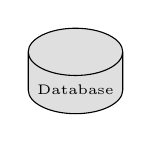
\begin{tikzpicture}[shape aspect=.5]
        \tikzset{every node/.style={cylinder,shape border rotate=90, draw,fill=gray!25}}
        \node at (1.5,0) {\shortstack{{{\tiny Database}}}};
       \end{tikzpicture}
    }}
    \newinst[2]{kyc}{\shortstack{KYC provider \\
       \\ 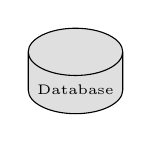
\begin{tikzpicture}[shape aspect=.5]
        \tikzset{every node/.style={cylinder,shape border rotate=90, draw,fill=gray!25}}
        \node at (1.5,0) {\shortstack{{{\tiny Database}}}};
       \end{tikzpicture}
    }}

    \postlevel
    \mess[0]{wallet}{{Initial action}}{exchange}
    \begin{callself}{exchange}{Establish KYC requirement}{}
    \end{callself}
    \mess[0]{exchange}{Request new KYC process}{kyc}
    \mess[0]{kyc}{{Process identifier (PI)}}{exchange}
    \mess[0]{exchange}{{KYC required (PI)}}{wallet}
    \mess[0]{wallet}{{KYC start (PI)}}{kyc}
    \mess[0]{kyc}{{Request identity documentation}}{wallet}
    \mess[0]{wallet}{{Upload identity documentation}}{kyc}
    \begin{callself}{kyc}{Validate documentation}{}
    \end{callself}
    \mess[0]{kyc}{{Share documentation (PI)}}{exchange}
    \mess[0]{kyc}{{Confirm completion}}{wallet}
    \mess[0]{wallet}{{Retry action}}{exchange}
\end{sequencediagram}
  \caption{Deposit interactions between customer, Taler exchange (payment
    service provider) and external KYC provider.  The process can be
    triggered by various {\em actions} described in Chapter~\ref{chap:triggers}.}
  \label{fig:proc:kyc}
\end{figure}

At the beginning of the KYC process, the user needs to specify whether they
are an {\bf individual} or a {\bf business}.\footnote{ In practice, we expect
most wallet-users to be individuals, but in principle a wallet could be owned
by a business.}  This then determines which types of attributes are collected
in the KYC process (Table~\ref{table:proc:kyc:individual} vs.
Table~\ref{table:proc:kyc:business}).

\begin{table}
  \caption{Information collected for individuals}
  \label{table:proc:kyc:individual}
  \begin{center}
    \begin{tabular}{l|c|r}
      {\bf Type}                 & {\bf Required}    & {\bf Example} \\ \hline \hline
      Surname                    & yes        & Mustermann \\
      First name(s)              & yes        & Max \\
      Date of birth              & yes        & 1.1.1980 \\
      Nationality                & yes        & Swiss \\
      Actual address of domicile & yes        & Seestrasse 3, 8008 Zuerich \\
      Phone number               & no         & +41-123456789 \\
      E-mail                     & no         & me@example.com \\
      Identification document    & yes        & JPG image \\
  \end{tabular}
  \end{center}
\end{table}

\begin{table}
  \caption{Information collected for businesses}
  \label{table:proc:kyc:business}
  \begin{center}
    \begin{tabular}{l|c|r}
      {\bf Type}                      & {\bf Required} & {\bf Example}        \\ \hline \hline
      Company name                    & yes        & Mega AG \\
      Registered office               & yes        & Seestrasse 4, 8008 Zuerich \\
      Company identification document & yes        & PDF file \\ \hline
      Contact person name             & yes        & Max Mustermann \\
      Phone number                    & no         & +41-123456789  \\
      E-mail                          & yes        & me@example.com \\
      Identification document         & yes        & JPG image \\
      Date of birth                   & yes        & 1.1.1980  \\
      Nationality                     & yes        & Swiss     \\ \hline
      Power of attorney arrangement   & yes        & PDF file  \\
  \end{tabular}
  \end{center}
\end{table}

\section{KYB process} \label{sec:proc:kyb}

\begin{figure}[h!]
  \begin{sequencediagram}
    \newinst{merchant}{\shortstack{Merchant \\
      \\ 
\begin{tikzpicture}
        \node [fill=gray!20,draw=black,thick,align=center] { Unique \\ Action};
      \end{tikzpicture}
    }}
    \newinst[2]{exchange}{\shortstack{Taler (exchange) \\
       \\ 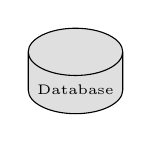
\begin{tikzpicture}[shape aspect=.5]
        \tikzset{every node/.style={cylinder,shape border rotate=90, draw,fill=gray!25}}
        \node at (1.5,0) {\shortstack{{{\tiny Database}}}};
       \end{tikzpicture}
    }}
    \newinst[2]{kyb}{\shortstack{KYB provider \\
       \\ 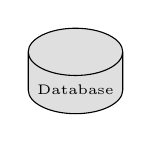
\begin{tikzpicture}[shape aspect=.5]
        \tikzset{every node/.style={cylinder,shape border rotate=90, draw,fill=gray!25}}
        \node at (1.5,0) {\shortstack{{{\tiny Database}}}};
       \end{tikzpicture}
    }}

    \postlevel
    \mess[0]{merchant}{{Initial action}}{exchange}
    \begin{callself}{exchange}{Establish KYB requirement}{}
    \end{callself}
    \mess[0]{exchange}{Request new KYB process}{kyb}
    \mess[0]{kyb}{{Process identifier (PI)}}{exchange}
    \mess[0]{exchange}{{KYB required (PI)}}{merchant}
    \mess[0]{merchant}{{KYB start (PI)}}{kyb}
    \mess[0]{kyb}{{Request identity documentation}}{merchant}
    \mess[0]{merchant}{{Upload identity documentation}}{kyb}
    \begin{callself}{kyb}{Validate documentation}{}
    \end{callself}
    \mess[0]{kyb}{{Share documentation (PI)}}{exchange}
    \mess[0]{kyb}{{Confirm completion}}{merchant}
    \mess[0]{merchant}{{Retry action}}{exchange}
\end{sequencediagram}
  \caption{Deposit interactions between customer, Taler exchange (payment
    service provider) and external KYB provider.  The process can be
    triggered by various {\em actions} described in Chapter~\ref{chap:triggers}.}
  \label{fig:proc:kyb}
\end{figure}

At the beginning of the KYB process, the user needs to specify whether they
are an {\bf individual} (not incorporated) or a {\bf business}.\footnote{In
practice, we expect most owners of bank accounts crossing the KYB threshold to
be businesses, but in principle such a bank account could be owned by an
individual operating a business without a separate legal entity.}  This then
determines which types of attributes are collected in the KYB process
(Table~\ref{table:proc:kyb:individual}
vs. Table~\ref{table:proc:kyb:business}).

\begin{table}
  \caption{Information collected for unincorporated individuals}
  \label{table:proc:kyb:individual}
  \begin{center}
    \begin{tabular}{l|c|r}
      {\bf Type}                 & {\bf Required}    & {\bf Example} \\ \hline \hline
      Surname                    & yes        & Mustermann \\
      First name(s)              & yes        & Max \\
      Date of birth              & yes        & 1.1.1980 \\
      Nationality                & yes        & Swiss \\
      Actual address of domicile & yes        & Seestrasse 3, 8008 Zuerich \\
      Phone number               & no         & +41-123456789 \\
      E-mail                     & no         & me@example.com \\
      Identification document    & yes        & JPG image \\
      Taxpayer identification    & yes        & ZPV Nr. 253'123'456 \\
  \end{tabular}
  \end{center}
\end{table}


\begin{table}
  \caption{Information collected for businesses. Information on individals is
    collected for owners with more than 25\% ownership and for those with
    signature authority for the business.}
  \label{table:proc:kyb:business}
  \begin{center}
    \begin{tabular}{l|c|r}
      {\bf Type}                        & {\bf Required} & {\bf Example}        \\ \hline \hline
      Company name                      & yes        & Mega AG \\
      Registered office                 & yes        & Seestrasse 4, 8008 Zuerich \\
      Company identification document   & yes        & PDF file \\
      Power of attorney arrangement     & yes        & PDF file  \\
      Business registration number      & yes        &  \\
      Business registration document    & yes        & PDF file \\
      Registration authority            & yes        &  \\ \hline
      Authorized person name            & yes        & Max Mustermann \\
      Share/authorization certification & yes        & PDF file \\
      Identification document           & yes        & JPG image \\
      Date of birth                     & yes        & 1.1.1980  \\
      Nationality                       & yes        & Swiss     \\
      E-mail                            & yes        & me@example.com \\
      Phone number                      & no         & +41-123456789  \\
  \end{tabular}
  \end{center}
\end{table}

\section{AML process}

\begin{figure}[h!]
  \begin{sequencediagram}
    \newinst{wallet}{\shortstack{Customer \\
      \\ 
\begin{tikzpicture}
        \node [fill=gray!20,draw=black,thick,align=center] { Unique \\ Action};
      \end{tikzpicture}
    }}
    \newinst[2]{exchange}{\shortstack{Taler (exchange) \\
       \\ 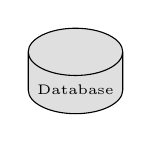
\begin{tikzpicture}[shape aspect=.5]
        \tikzset{every node/.style={cylinder,shape border rotate=90, draw,fill=gray!25}}
        \node at (1.5,0) {\shortstack{{{\tiny Database}}}};
       \end{tikzpicture}
    }}
    \newinst[2]{staff}{\shortstack{AML staff \\
      \\ 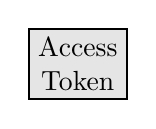
\begin{tikzpicture}
        \node [fill=gray!20,draw=black,thick,align=center] { Access \\ Token};
      \end{tikzpicture}
    }}
    \postlevel
    \mess[0]{wallet}{{Initial action}}{exchange}
    \begin{callself}{exchange}{Establish AML requirement}{}
    \end{callself}
    \begin{callself}{exchange}{Queue AML task}{}
    \end{callself}
    \mess[0]{exchange}{Wait for AML}{wallet}
    \mess[0]{staff}{Request AML work}{exchange}
    \mess[0]{exchange}{{Open AML task(s)}}{staff}
    \mess[0]{staff}{Request details}{exchange}
    \mess[0]{exchange}{KYC/AML data}{staff}
    \begin{callself}{staff}{Review and decide}{}
    \end{callself}
    \mess[0]{staff}{{Decision documentation}}{exchange}
    \mess[0]{exchange}{AML decision}{wallet}
    \mess[0]{wallet}{{Retry action}}{exchange}
\end{sequencediagram}
  \caption{Deposit interactions between customer, Taler exchange (payment
    service provider) and the AML staff.  The process can be
    triggered by various {\em actions} described in Chapter~\ref{chap:triggers}.
    AML staff interactions are cryptographically secured and
    decisions and the provided reasoning are archived by the exchange.
    AML staff may interact with the customer (out-of-band)
    in its decision process.
    }
  \label{fig:proc:aml}
\end{figure}


\chapter{Fees} \label{chap:fees}

The business model for operating a Taler exchange is to charge transaction
fees.  Fees are charged on certain operations by the exchange.  There are two
types of fees, {\bf wire fees} and {\bf coin fees}.  This chapter describes
the fee structure.

Fixed, amount-independent {\bf wire fees} are charged on wire transfers using
the core banking system.  Details on wire fees are described in
Section~\ref{sec:fees:wire}.

Coin fees are more complex, as they do not exactly follow neither the usual
percentage of volume model of other payment systems.  Instead, coin fees are
applied per coin, resulting in a {\em logarithmic} fee structure.  As a
result, the effective fee {\em percentage} for tiny transactions is high (for
example 50\% for transactions of 0.0025 CHF) while the effective fee
percentage for large transactions is nominal (for example $\approx$ 0.05\% for
transactions of $\approx$ 40 CHF). Details on coin fees are described in
Section~\ref{sec:fees:coin}.

Fees are configurable (and that fee types beyond those described here are
supported by the software). Thus, the specific fees may be adjusted in the
future based on business decisions.  However, changes to the fees are never
retroactively applied to coins already in circulation.  Wire fees that have
been publicly announced for a particular time period also cannot be changed.
Finally, any change to the terms of service must also be explicitly accepted
by the users before they withdraw additional funds.


\section{Fees per wire} \label{sec:fees:wire}

Wire fees apply whenever an exchange needs to initiate a wire transfer to
another bank account.  Wire fees do not apply to every individual payment to a
merchant, as merchants can choose to {\em aggregate} multiple micropayments
into one large payment on the wire.  Wire fees also do not apply to
wallet-to-wallet payments within the Taler system.

A {\bf wire} fee is applied when a merchant receives
an aggregated payment into their bank account.

A {\bf closing} fee is applied when a wallet fails to
withdraw coins and money has to be sent back to the
originating bank account.

\begin{table}[h!]
  \caption{Table with wire fees. Wire fees are set annually.}
  \label{table:fees:wire}
  \begin{center}
    \begin{tabular}{l|c|r}
      {\bf Year} & {\bf Fee type} & {\bf Amount}   \\ \hline \hline
      2023       & wire           & {\em CHF 0.05} \\
      2023       & closing        & {\em CHF 0.10} \\
      2024       & wire           & {\em CHF 0.05} \\
      2024       & closing        & {\em CHF 0.10} \\
      2025       & wire           & {\em CHF 0.05} \\
      2025       & closing        & {\em CHF 0.10} \\
  \end{tabular}
  \end{center}
\end{table}

\section{Fees per coin} \label{sec:fees:coin}

Payments with Taler are always made using coins.  Each coin has a specific
denomination, and an exchange will issue coins in different denominations (in
the same currency).  The fees per coin depend on the operation and the
denomination.

The primary fee to be paid is a {\bf deposit} fee that is
charged whenever a coin is fully or partially deposited
into a bank account or another wallet.

A secondary fee to be paid is a {\bf change} fee that is
charged whenever a coin partially spent and change must
be rendered.

Coins also have an {\bf expiration} date of approximately {\bf one year}.
After the expiration date, coins become worthless.  Wallets that are online
{\bf three months} {\em before} a coin expires will automatically trade any
such coins for one or more fresh coins with a later expiration date. This
process is also subject to the {\bf change} fee.


\begin{table}[h!]
  \caption{Fees per coin. Coin denomination values are given in units of CHF 0.01.}
  \label{table:fees:coins}
  \begin{center}
    \begin{tabular}{l|c|r}
      {\bf Denomination} & {\bf Fee type} & {\bf Amount}   \\ \hline \hline
     $2^{-4}-2^{ 0}$      & deposit        & {\em CHF 0.00125} \\
     $2^{-4}-2^{ 0}$      & change         & {\em CHF 0.00125} \\
     $2^{ 0}-2^{ 3}$      & deposit        & {\em CHF 0.00250} \\
     $2^{ 0}-2^{ 3}$      & change         & {\em CHF 0.00125} \\
     $2^{ 4}-2^{ 8}$      & deposit        & {\em CHF 0.005} \\
     $2^{ 4}-2^{ 8}$      & change         & {\em CHF 0.00125} \\
     $2^{ 8}-2^{12}$      & deposit        & {\em CHF 0.01} \\
     $2^{ 8}-2^{12}$      & change         & {\em CHF 0.00125} \\
    \end{tabular}
  \end{center}
\end{table}

%\include{fees-other}


\end{document}
